\documentclass[11pt]{article}
\usepackage{acl2014}
\usepackage{times}
\usepackage{url}
\usepackage{latexsym}
\usepackage{graphicx}
\usepackage{array}

\newcolumntype{L}[1]{>{\raggedright\let\newline\\\arraybackslash\hspace{0pt}}m{#1}}

\title{Analyzing Helpfulness of Amazon Reviews}
\date{\today}

\author{
  \textbf{Yuliana Havryshchuk} \\
    \tt{yuliana.havryshchuk@epfl.ch} \\
  \textbf{Jonathan Donas} \\
    \tt{jonathan.donas@epfl.ch} \\
  \textbf{Julien Harbulot} \\
    \tt{julien.harbulot@epfl.ch}}

\begin{document}
\maketitle
\begin{abstract}

This project investigates what makes an Amazon review helpful. We explored the relationships between helpfulness and length, star-rating, words used, and trends over time. We found that the review length, star-rating, and the words used in a review were the most telling factors. Furthermore, a new classifier is not necessarily needed for each product category. We found that the same words that indicate that a beauty product review is helpful can also tell us if an automotive product or baby product review is helpful.

\end{abstract}

\vspace{0em}
\section{Introduction}

Useful reviews are important to Amazon because they help customers make informed decisions about which products to buy. If a customer finds a product from an unknown company, they are much more likely to buy it if it has already been vetted by other users - as opposed to if there are no reviews. Even better, a helpful review can push a customer to make a purchase when he or she is on the fence.

Currently, Amazon uses a user voting system to determine which reviews are the most helpful and should be displayed at the top of the list. A user can vote "Yes" or "No" about the helpfulness of reviews that they see on the site. With this project, we aimed to identify what makes reviews helpful or unhelpful, and identify if a review is helpful automatically: without the use of user-voting.

\vspace{0.5em}
\section{Data Collection}

We chose to use the amazon review data-set.\footnote{http://jmcauley.ucsd.edu/data/amazon/} We compiled the statistics on 5 product categories (beauty, automotive, electronics, baby, books) but narrowed our focus to the automotive, beauty, and books data-sets. The purpose of this was to test our hypothesis that different product categories needed different classifiers to determine helpfulness. In each category, we only took products with between 50 and 100 reviews, and then only took reviews with over 10 votes of helpfulness. 

We also analyzed data of customers who have left at least 150 reviews on the website, and took their reviews with at least 30 votes. The columns in our data that were most useful for analysis were: \textit{}{review\_body}, \textit{review\_date}, \textit{star\_rating}, \textit{helpful\_votes}, and \textit{total\_votes}.

\vspace{0.5em}
\section{Data-Set Description}

Automotive:
\vspace{-0.8em}
\begin{itemize}
\itemsep-0.4em
\item Count: \textbf{14 557}
\item Reviews that are helpful: \textbf{74\%}
\item Average helpfulness score: \textbf{83\%}
\end{itemize}

\noindent Beauty:
\vspace{-0.8em}
\begin{itemize}
\itemsep-0.4em
\item Count: \textbf{35 571}
\item Reviews that are helpful: \textbf{69.5\%}
\item Average helpfulness \%: \textbf{83\%}
\end{itemize}

\noindent Books:
\vspace{-0.8em}
\begin{itemize}
\itemsep-0.4em
\item Count: \textbf{316 018}
\item Reviews that are helpful: \textbf{47.5\%}
\item Average helpfulness \%: \textbf{70\%}
\end{itemize}

\noindent Most Frequent Reviewers:
\vspace{-0.8em}
\begin{itemize}
\itemsep-0.4em
\item Count: \textbf{219 566}
\item Reviews that are helpful: \textbf{75.9\%}
\item Average helpfulness \%: \textbf{83\%}
\end{itemize}

\vspace{0em}
\section{Description of Main Algorithms}

Deciding what "helpful" meant was difficult. If we define a review as helpful if 50\% of voters say "yes", then 94\% of reviews turn out to be helpful and we can also classify the helpful reviews with an accuracy of 94\%. But that would not be very useful for Amazon, because it needs to know the top reviews. We decided to define helpfulness as 80\% of people voting a review to be helpful.

To pre-process reviews for classification, we took the review body and removed punctuation, removed stop-words (using the nltk library list with a few modifications), removed words shorter than 4 characters, and tokenized the review body texts.

We first tried Multinomial Naive Bayes classifier. Then we tried a Compliment Naive Bayes classifier because it is well-suited for imbalanced data sets. When we examined our data, we saw that reviews were skewed towards being helpful. 

\vspace{0.5em}
\section{Results and Findings}

\subsection{Review Length vs. Helpfulness}
In all of the product categories, helpful reviews were longer than unhelpful reviews. The average length of helpful review is 763, compared to the average length of unhelpful reviews at 598. Clearly, the longer a review is, the more likely it is to have a high helpfulness score. 

\begin{figure}[!htb]
\fbox{
    \begin{minipage}{\dimexpr\linewidth-2ex\relax}
    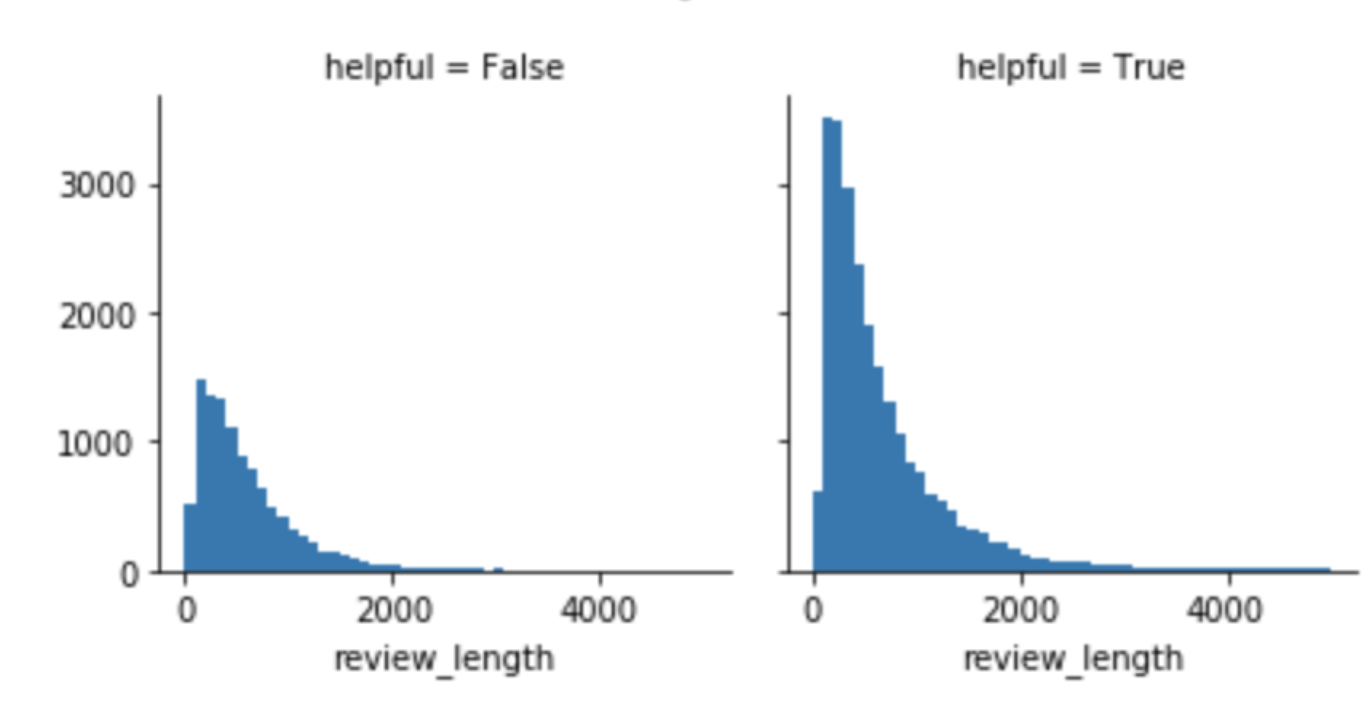
\includegraphics[width=\dimexpr\linewidth-2ex\relax]{Image1.png}
    \end{minipage}
}
\begin{center}
Figure 5.1.1
\end{center}
\end{figure}

\begin{figure}[!htb]
\fbox{
    \begin{minipage}{\dimexpr\linewidth-2ex\relax}
    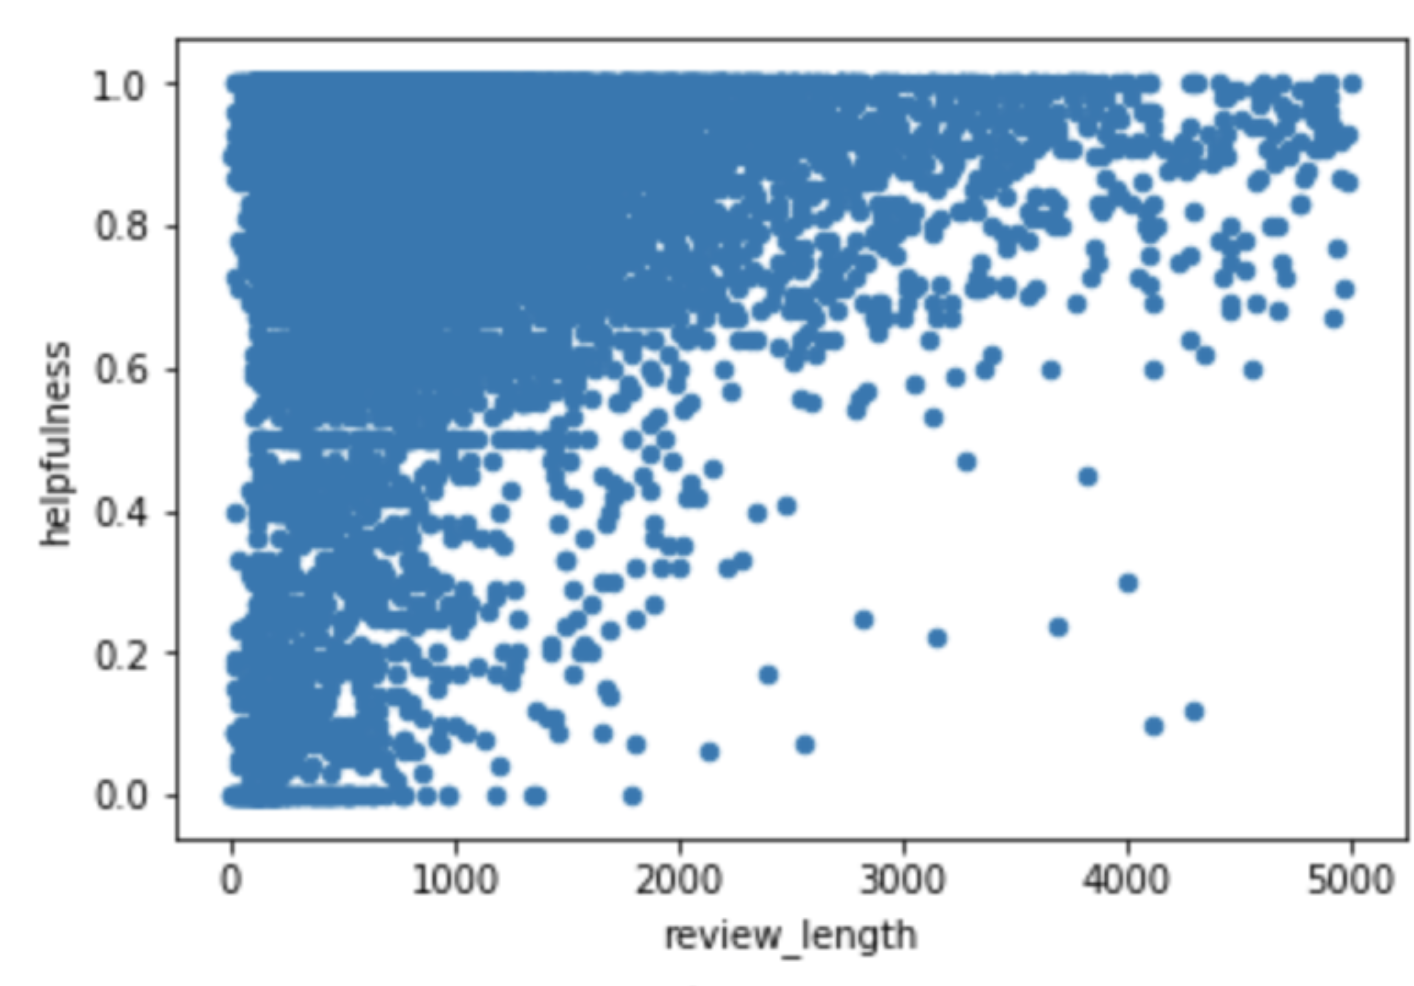
\includegraphics[width=\dimexpr\linewidth-2ex\relax]{Image2.png}
    \end{minipage}
}
\begin{center}
Figure 5.2.2
\end{center}
\end{figure}

\subsection{Verified/Unverified vs. Helpfulness}

Reviews that were written by people whose purchase was Amazon verified were not more helpful than non-verified purchases. There was often less than 2\% difference between the two, and sometimes, with non-verified purchases having higher reviews. The conclusion to take from this is that unverified reviewers have indeed actually tried the product at some point, since they have meaningful comments about it.

\subsection{Star Rating vs. Helpfulness}

There is a common pattern between all five product categories with respect to the relationship between a review’s star rating, and its helpfulness. First of all, as expected, most reviews give either 1 or 5 stars. For unhelpful reviews, the more common star-rating is 1-star, by about 50\%. For helpful reviews, the most common star-rating is by far 5-stars. We were surprised by this because our intuition said that 3 and 4 star reviews would be most helpful because the extreme ratings might be emotionally charged, whereas a medium rating would be more rational and include helpful pros and cons of a product. We think that 5-star reviews were more likely to be helpful because people like to feel good about the product they want to buy, and 5-star reviews reinforce that. The relationship between stars and helpfulness is not strong enough for us to use it as a predictor.

\begin{figure}[!htb]
\fbox{
    \begin{minipage}{\dimexpr\linewidth-2ex\relax}
    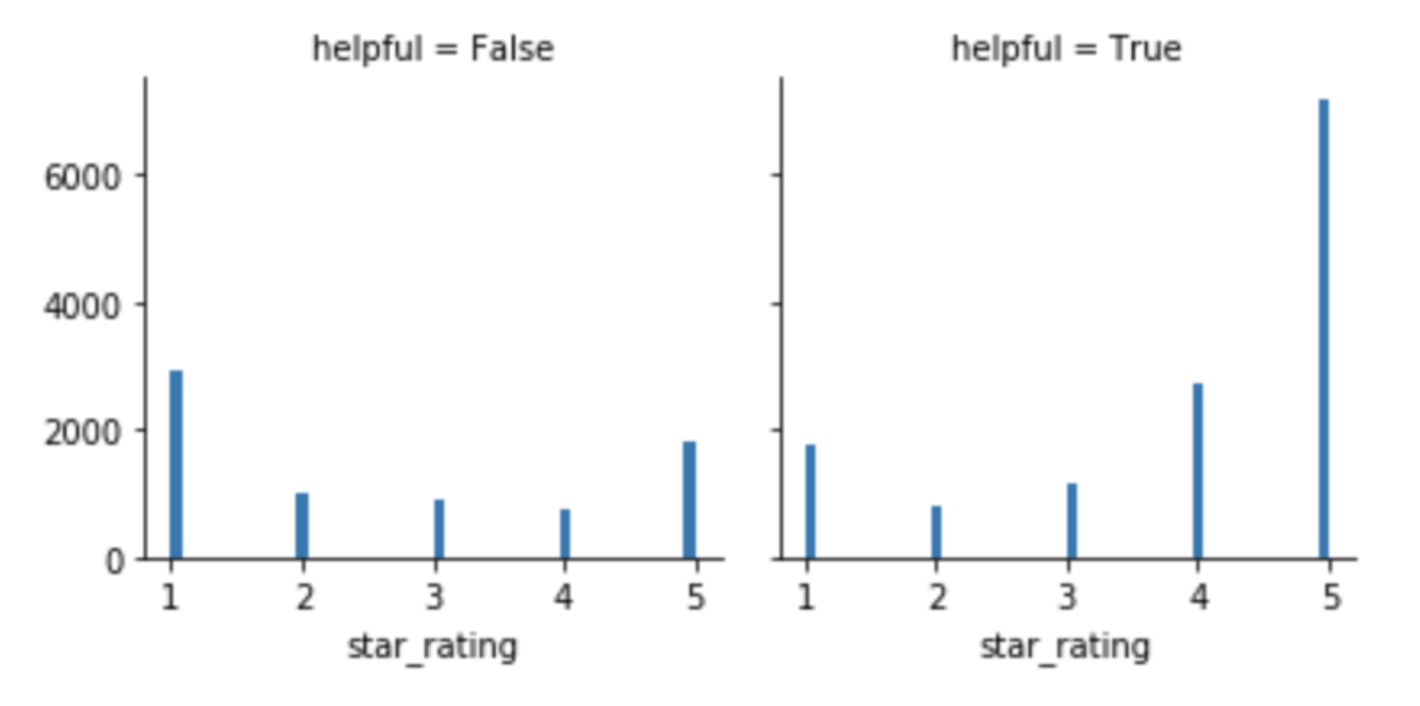
\includegraphics[width=\dimexpr\linewidth-2ex\relax]{Image3.png}
    \end{minipage}
}
\begin{center}
Figure 5.3.1
\end{center}
\end{figure}

\subsection{Customer Review Helpfulness Over Time}

We also wanted to see if there was a trend in review helpfulness over time, and we did see an interesting pattern. The oldest data available, from around 2000, has almost no unhelpful reviews. It took about 4 years for the distribution to balance out a bit. Then, as time went on to 2016, the extremes became more saturated. It is more likely for a review to be 90-10\% helpful or 0-10\% helpful than it is for a review to be 40-50\% helpful. 

\begin{figure}[!htb]
\fbox{
    \begin{minipage}{\dimexpr\linewidth-2ex\relax}
    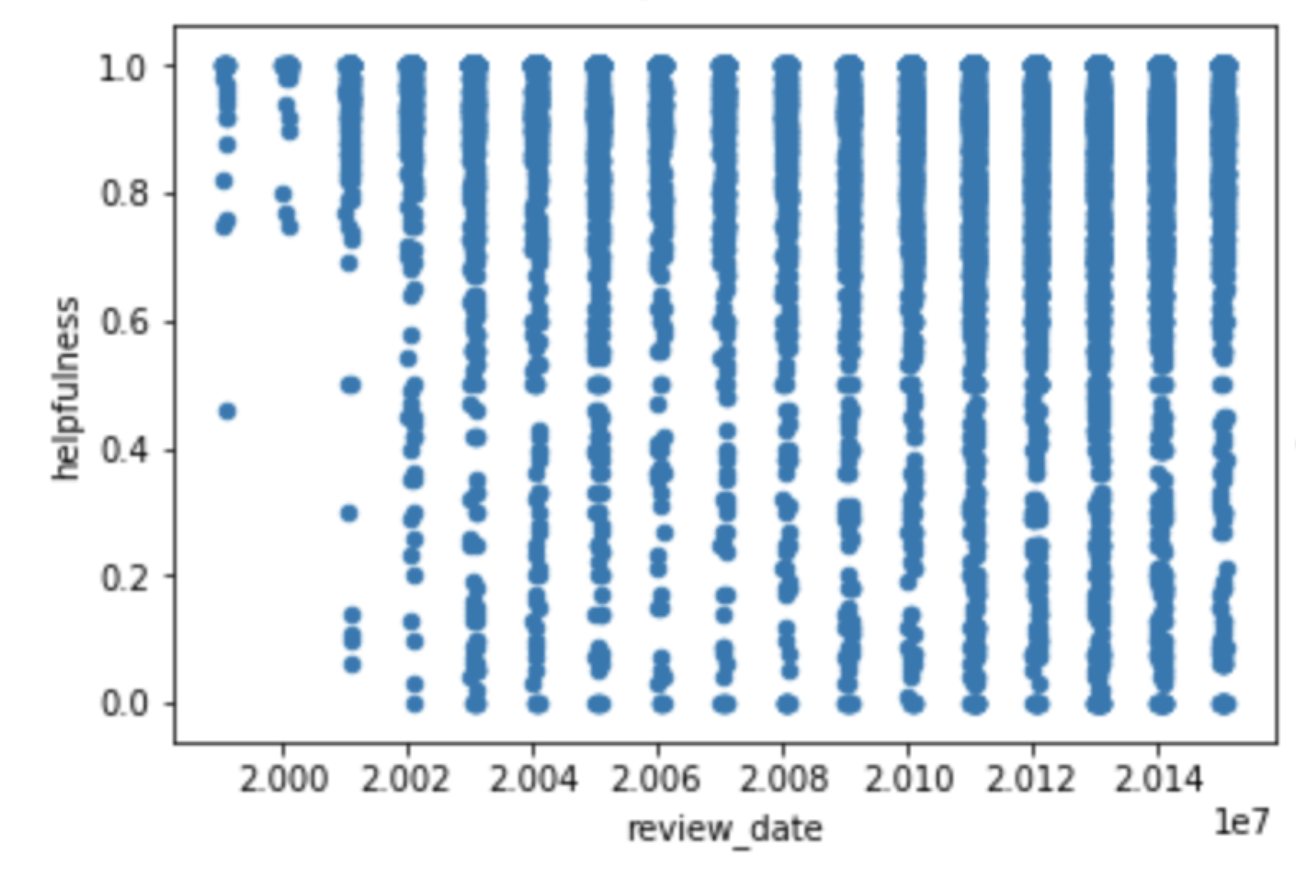
\includegraphics[width=\dimexpr\linewidth-2ex\relax, height=4.5cm]{Image4.png}
    \end{minipage}
}
\begin{center}
Figure 5.4.1
\end{center}
\end{figure}

\subsection{Frequent Reviewers}

To explore individual reviewers further, we looked at data for customers who had left over 150 reviews on Amazon. We hypothesized that their review helpfulness would be much higher, and most likely improve over time. We found that to not be the case at all (only true for one of the top 10 reviewers). Each one had a different pattern when we examined their review helpfulness over time. Some reviewers had all of their reviews voted as extremely useful, whereas other reviewers had no pattern at all — the review was just as likely to be 10\% helpful as it was to be 90\% helpful. This information makes sense when we look at the average helpfulness rating overall, and the average helpfulness rating of frequent reviewers (they are both around 83\%). It seems like Amazon reviews are like twitter — just because there is a lot of activity does not mean that it is quality content. 

One big difference between these reviews and the overall data-set is that the length of the reviews is much longer. Overall, the average length of a helpful review is 763 and the average length of an unhelpful review is 598. For frequent reviewers, average length of a helpful review is 1952, and the average length of an unhelpful review is 1573. They are over 2x longer. This makes sense because these people have shown that they have time and effort to put into reviews, but it still does not help us classify helpful reviews.

\begin{figure}[!htb]
\fbox{
    \begin{minipage}{\dimexpr\linewidth-2ex\relax}
    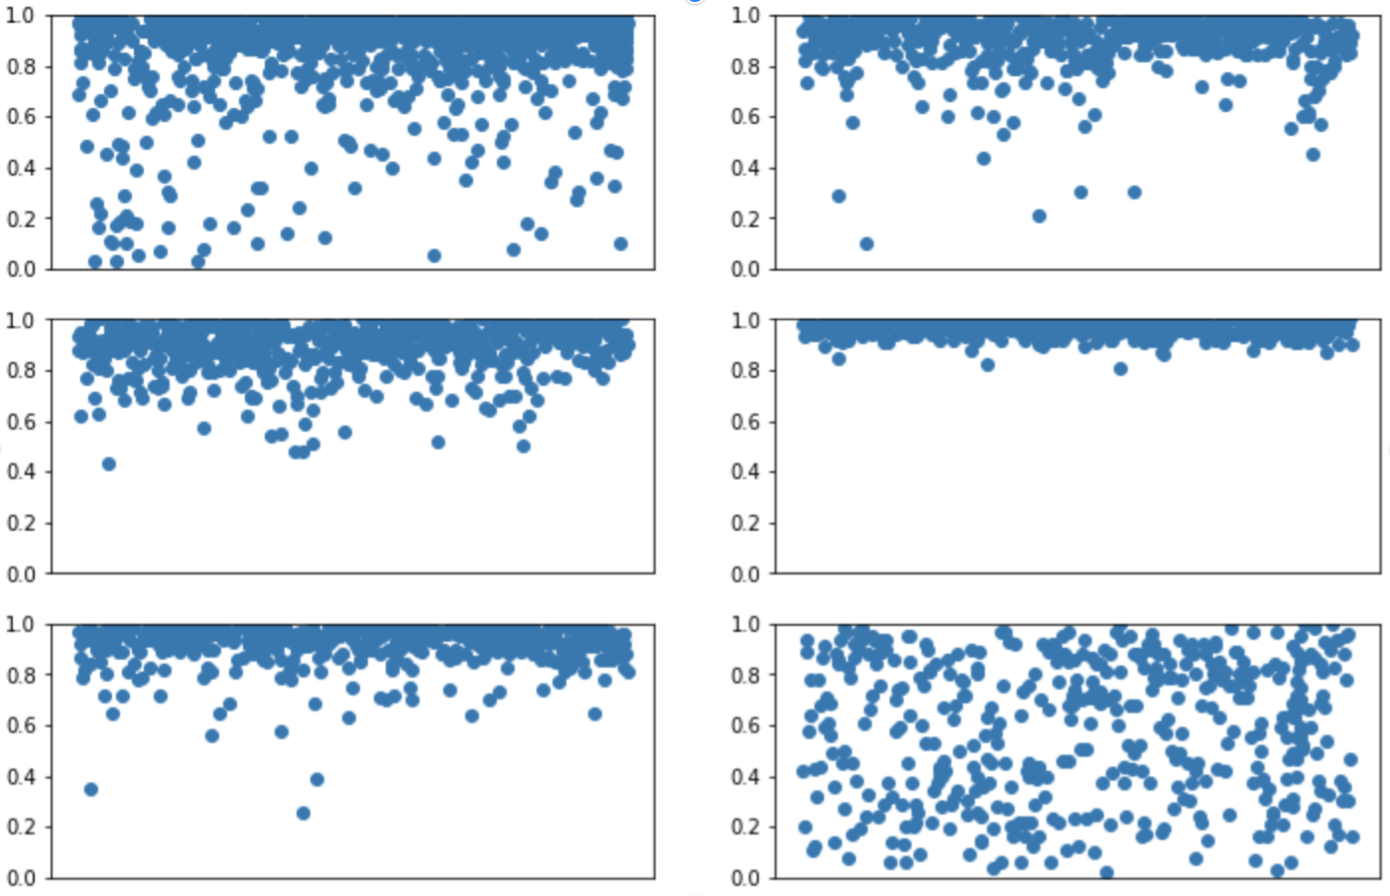
\includegraphics[width=\dimexpr\linewidth-2ex\relax]{Image5.png}
    \end{minipage}
}
\begin{center}
Figure 5.5.1
\end{center}
\end{figure}

\subsection{Classifying Helpfulness Based on Review Body Text}

Finally, the last experiments we did were to see if we can predict whether a review is helpful or not based on the words used in the review. We were able to predict helpful reviews with an accuracy of 85\% after the pre-processing described above. Using Complement Naive Bayes only gave a 1\% improvement over Multinomial Naive Bayes, which was surprising because of our data-set imbalance.

Using Complement Naive Bayes did not always give our predictor an improvement, which was surprising because of our data-set imbalance. In most cases, using Complement made the results worse. We expected to see that there would be a big improvement of predicting False (unhelpful reviews), but that was not the case. 

\begin{center}
\begin{tabular}{|p{1.8cm}|L{2.3cm}|L{2.3cm}| } 
\hline
& Precision (Multivariate NB) & Precision (Complement NB) \\
\hline
Automotive & \shortstack[l]{false: 0.53 \\ true: 0.79 \\ weighted: 0.73} & \shortstack[l]{false: 0.53 \\ true: 0.79 \\ weighted: 0.73} \\
\hline
Baby & \shortstack[l]{false: 0.53 \\ true: 0.79 \\ weighted: 0.73} & \shortstack[l]{false: 0.53 \\ true: 0.79 \\ weighted: 0.73} \\
\hline
Beauty & \shortstack[l]{false: 0.53 \\ true: 0.79 \\ weighted: 0.73} & \shortstack[l]{false: 0.53 \\ true: 0.79 \\ weighted: 0.73} \\
\hline
Electronics & \shortstack[l]{false: 0.53 \\ true: 0.79 \\ weighted: 0.73} & \shortstack[l]{false: 0.53 \\ true: 0.79 \\ weighted: 0.73} \\
\hline
\end{tabular}
\end{center}
\vspace*{10px}

Additionally, we were surprised that using a classifier trained on one product category was not at all worse when used on other categories. In fact, sometimes the test set from a different category was more accurately predicted. This makes sense because negative and positive words are not necessarily related to the product category. Positive words like “perfect, good value, repurchase”  can be applied to any product, similar to negative words like “cheap, broken, useless”.

\vspace*{10px}
\begin{center}
\begin{tabular}{|p{1.4cm}|L{1.5cm}|L{1.5cm}|L{1.5cm}| } 
\hline
& Beauty w/ beauty classifier & Auto w/ auto classifier & Auto w/ beauty classifier \\
\hline
Precision (False) & 0.52 & 0.53 & 0.43 \\
\hline
Precision (True) & 0.74 & 0.79 & 0.76 \\
\hline
Precision (weighted average) & 0.67 & 0.73 & 0.68 \\ 
\hline
\end{tabular}
\end{center}
\vspace*{10px}

Next, we decided to try to fix the imbalance in the data. We needed to create a data-set that sampled many more unhelpful reviews, because so far, the ratio of helpful to unhelpful was 3:17. To create this modified data-set, we used the Books category reviews. We removed the middle tier reviews, and focused on the extremes. We took reviews that scored 0-20\%, or 99-100\% helpfulness. Finally, one of our hypotheses was confirmed, and we got much better results. We got an accuracy of 89\% for unhelpful reviews, and 78\% for helpful reviews. It is now much easier to identify an unhelpful review, which is the opposite of the case when we include all of the data - even though the number of helpful reviews still outweighed the unhelpful. This shows us that we can get a much higher accuracy for all of the categories if we train our classifiers on balanced data. It is also much easier to classify reviews at the extremes, for obvious reasons. 

\section{Conclusion}

Our initial data-set had a much higher number of helpful reviews than unhelpful reviews. This means that the model is more biased towards useful reviews compared to useless ones.

Although our model was biased towards helpful reviews, it was relatively accurate with its predictions and achieved an accuracy of up to 80\% on the helpful reviews in some test sets. However, it was not good at classifying unhelpful reviews, with an accuracy of up to 60\%. Our results were much better when we used under-sampling to achieve a balance in the Books data-set so that the classifier would be better able to detect unhelpful reviews. 

With fairly simple models, we can do a good job of automatically predicting whether an amazon review is helpful or not. Additional research can be done to utilize the length, date, and star rating of reviews to improve the classifier. 

\end{document}
